\documentclass{article}
\usepackage{graphicx} % Required for inserting images
\usepackage[left=1.5cm, right=1.5cm, top=1.5cm]{geometry}
\usepackage{enumitem}
\usepackage{amsmath}
\usepackage{amsfonts}
\usepackage{listings}
\usepackage{xcolor}

\definecolor{dkgreen}{rgb}{0,0.6,0}
\definecolor{mauve}{rgb}{0.58,0,0.82}
\usepackage[utf8]{inputenc}

\lstset{frame=tb,
  language=Bash,
  aboveskip=3mm,
  belowskip=3mm,
  showstringspaces=false,
  columns=flexible,
  basicstyle={\small\ttfamily},
  numbers=none,
  numberstyle=\tiny\color{gray},
  keywordstyle=\color{blue},
  commentstyle=\color{dkgreen},
  stringstyle=\color{mauve},
  breaklines=true,
  breakatwhitespace=true,
  tabsize=4
}

\title{Distributed Systems: Assignment 2}
\author{Deven Mistry}
\date{Feb 19th, 2025}
\setlength\parindent{0pt}
\begin{document}

\maketitle

In this assignment, we create a kubernetes cluster, fire a shell in that cluster and forward a port to the system outside.

Steps involved in creating and installing the cluster were the most difficult for me as I couldn't find a starter image to instantiate the container. Upon going through the documentation on the `kubernetes' website, I found the yml file required to start the cluster. Once the container was fired up, the remaining process was pretty straightforward. Here are the steps, I followed.



\section*{Installing Docker, Kubernetes and minikube}

I installed Docker Desktop from the official website. To install `kubectl' and `minikube', I used the following commands.

\begin{lstlisting}
curl -LO "https://dl.k8s.io/release/$(curl -L -s https://dl.k8s.io/release/stable.txt)/bin/darwin/arm64/kubectl"
chmod +x ./kubectl
sudo mv ./kubectl /usr/local/bin/kubectl
\end{lstlisting}

To install minikube

\begin{lstlisting}
curl -LO https://github.com/kubernetes/minikube/releases/latest/download/minikube-darwin-arm64
sudo install minikube-darwin-arm64 /usr/local/bin/minikube
\end{lstlisting}

\section*{Starting the container}

To create the kubernetes container, I first started Docker, and then

\begin{lstlisting}
minikube start
kubectl create -f shell-demo.yml  # to create the container
kubectl get pods                     # to check if the container is running

# launch the container
kubectl exec -it shell-demo -- /bin/bash
\end{lstlisting}

\section*{Copying files to the container}

Using the command given in the assignment 1, I copied the files to the container.

% The command was `kubectl cp hw1 shell-demo:hw1'

\begin{lstlisting}
kubectl cp hw1 shell-demo:hw1
\end{lstlisting}

% \begin{enumerate}


%     \item The client sends a JSON message to the server. The client was tested using the `python client.py' command in the terminal.
%     \item The client sends a JSON message to the server using the requests library using a POST method.
% \end{enumerate}

\section*{Running server on the container and forwarding the port}

Once the files, were copied to the container, I ran the server using the command given in the assignment.

\begin{lstlisting}
kubectl exec -it shell-demo -- /bin/bash
cd hw1
python3 server.py
\end{lstlisting}

\section*{Running client locally}

In a different terminal, I just ran the client and sent a message to the server.

\begin{lstlisting}
python3 client.py
\end{lstlisting}

\section*{Screenshot of the output}

\begin{figure}[ht]
    \centering
    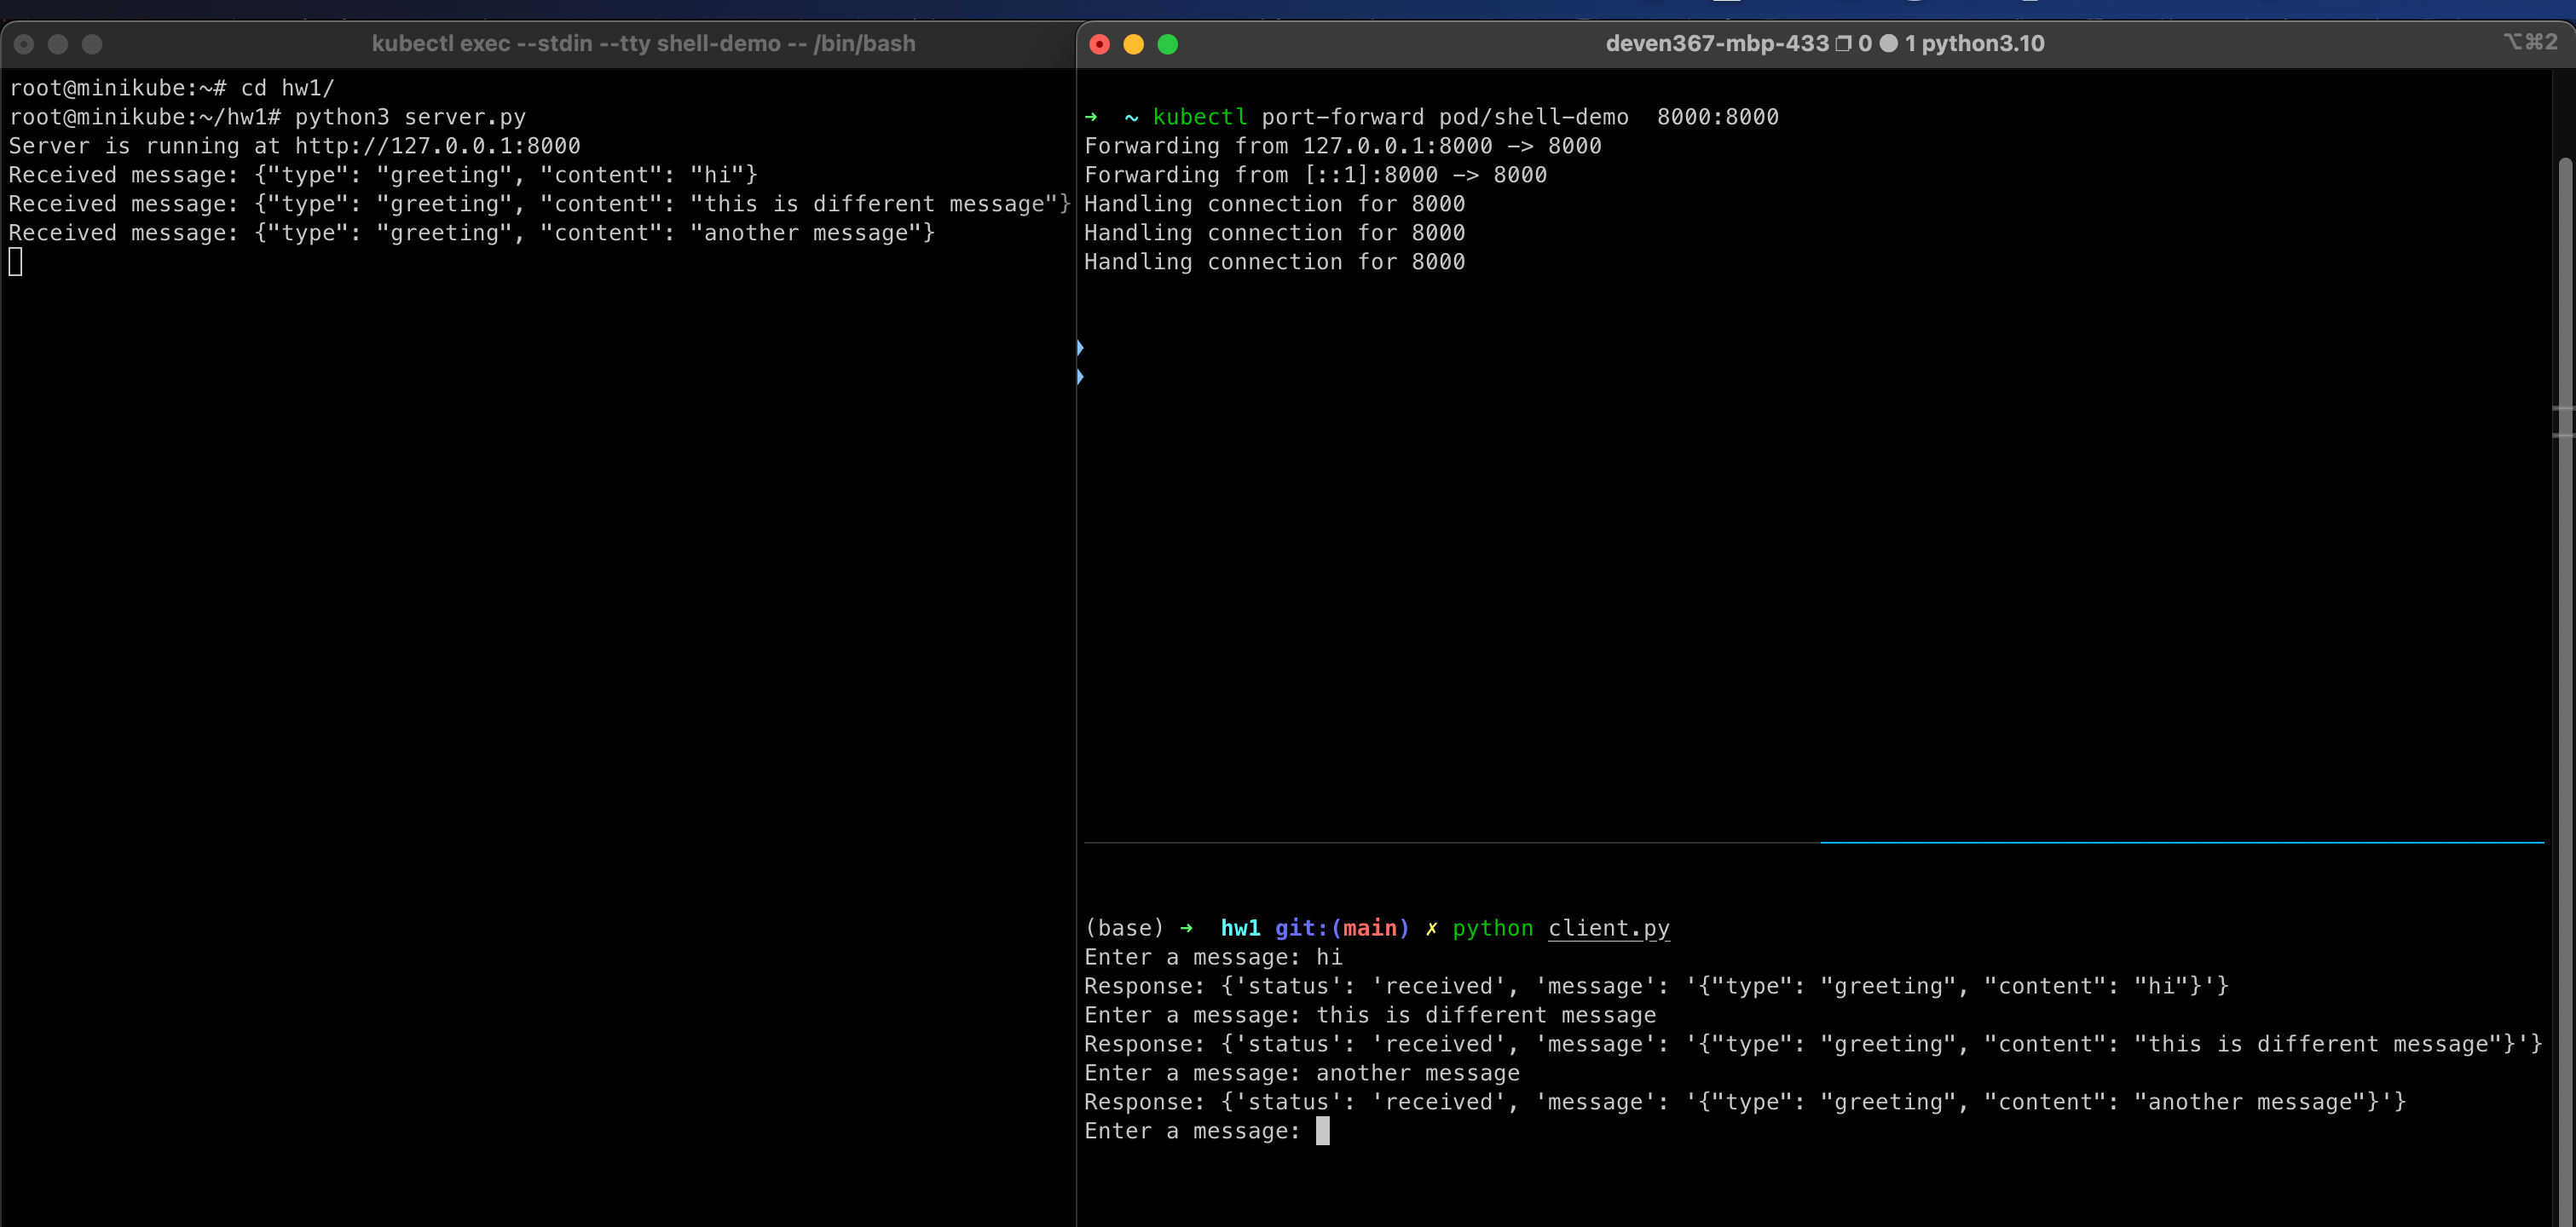
\includegraphics[width=0.8\textwidth]{output.png}
    \caption{Client communicating with the server running on the container from the forwarded port}
\end{figure}

\end{document}
